\documentclass[conference]{IEEEtran}
\usepackage{booktabs}
\usepackage{graphicx}
\usepackage{amsmath}
\usepackage{amssymb}
\usepackage{hyperref}
\usepackage{cite}
\usepackage{float}

\begin{document}

\title{Classical Baseline for Handwritten Short Answer Grading: A Statistical Lexical Approach on SciEntsBank}

\author{\IEEEauthorblockN{Udita}
\IEEEauthorblockA{Roll No: 230082 \\
NST, Rishihood University, Sonipat \\
Advanced Machine Learning}}

\maketitle

\begin{abstract}
The automated grading of handwritten student responses is a cornerstone problem in Educational Technology (EdTech), requiring a convergence of computer vision and natural language processing. This paper establishes a rigorous classical baseline for this task using the SciEntsBank dataset. We deploy a non-neural pipeline comprising Tesseract OCR (Legacy Engine, OEM 0) for transcription, followed by a statistical feature engineering layer utilizing TF-IDF and Jaccard similarity. Evaluation is performed across three critical dimensions: Unseen Answers (UA), Unseen Questions (UQ), and Unseen Domains (UD). Our results indicate that while lexical overlap models provide a strong initial benchmark (F1 Macro = 0.5732 on UA), they suffer from a significant "Semantic Gap" and "Domain Shift" (F1 Macro = 0.4974 on UD), establishing the theoretical and empirical motivation for neural semantic integration in subsequent phases.
\end{abstract}

\begin{IEEEkeywords}
Short Answer Grading, OCR, Tesseract, TF-IDF, SciEntsBank, Educational Technology.
\end{IEEEkeywords}

\section{Introduction}
Manual grading represents a bottleneck in pedagogical scaling. As student enrollment grows, the cognitive load on human graders increases, often leading to inconsistency and delayed feedback. Automated Short Answer Grading (ASAG) aims to mitigate this by providing instantaneous, objective evaluations.

However, ASAG remains a "wicked problem" due to:
\begin{enumerate}
    \item \textit{Lexical Variability}: Students may use synonyms (e.g., "power" instead of "energy") which lexical matchers fail to recognize.
    \item \textit{Noise Propagation}: Errors in Optical Character Recognition (OCR) directly degrade the downstream grading logic.
    \item \textit{Out-of-Distribution (OOD) Generalization}: Models often memorize domain-specific vocabulary rather than underlying scientific concepts.
\end{enumerate}

This Phase 1 report establishes a foundational non-neural baseline. We intentionally avoid deep learning techniques to isolate the performance of classical statistical methods, thereby creating a controlled environment for future ablation studies.

\section{Literature Review}
The study of automated grading is rooted in the "Student Response Analysis" task. Dzikovska et al. \cite{dzikovska2013} introduced the SciEntsBank dataset in the SemEval-2013 challenge, which has since become the gold standard for science domain ASAG.

Classical text retrieval foundations rely heavily on the Vector Space Model. Salton and Buckley \cite{salton1988} pioneered the TF-IDF (Term Frequency-Inverse Document Frequency) weighting scheme, which quantifies the informational significance of terms. Robertson and Zaragoza \cite{robertson2009} later refined this into the BM25 probabilistic framework.

Mohler and Mihalcea \cite{mohler2009} conducted a thorough survey of lexical similarity measures, highlighting that while set-based overlap (Jaccard) is efficient, it cannot bridge the semantic gap in student responses. Our baseline pairings — Tesseract \cite{smith2007} for transcription and Logistic Regression for classification — constitute a representative snapshot of pre-neural EdTech solutions.

\section{Methodology}
\subsection{The SciEntsBank Dataset}
The dataset is structured to test three levels of generalization:
\begin{itemize}
    \item \textbf{UA (Unseen Answers)}: Tests generalization to new phraseology for known questions.
    \item \textbf{UQ (Unseen Questions)}: Tests performance on new prompts within known science domains.
    \item \textbf{UD (Unseen Domains)}: Tests strictly OOD generalization to entirely new science topics (e.g., moving from biology to chemistry).
\end{itemize}

\subsection{OCR: Tesseract Legacy Architecture}
Transcription is handled via Tesseract's \texttt{--oem 0} engine. We chose the legacy engine over the newer LSTM-based engine (\texttt{--oem 3}) to maintain a pure non-neural baseline. Preprocessing involves:
\begin{enumerate}
    \item \textit{Grayscale Conversion}: $Y = 0.299R + 0.587G + 0.114B$.
    \item \textit{Autocontrast}: Histogram stretching to maximize dynamic range.
    \item \textit{Otsu Binarization}: Global thresholding to isolate ink from paper.
\end{enumerate}

\subsection{Feature Engineering and Rigor}
We model student responses in a high-dimensional sparsity-aware feature space.

\subsubsection{TF-IDF Formulation}
Each student answer $D$ is represented as a vector where the weight of term $t$ is:
\begin{equation}
w_{t,D} = \text{tf}_{t,D} \times \log\left(\frac{N}{\text{df}_t}\right)
\end{equation}
where $\text{tf}_{t,D}$ is the term frequency and $\text{df}_t$ is the number of documents containing $t$. This identifies discriminative scientific keywords.

\subsubsection{Jaccard Similarity}
To measure the surface-level structural overlap between the student answer ($S$) and reference answer ($R$), we use the Jaccard index:
\begin{equation}
J(S,R) = \frac{|S \cap R|}{|S \cup R|}
\end{equation}

\subsubsection{Token Density}
We calculate the recall-based overlap:
\begin{equation}
\delta = \frac{|S \cap R|}{|R|}
\end{equation}
This explicitly measures how much of the "gold standard" content were recovered by the student.

\subsection{Classification: Softmax Logistic Regression}
We deploy a Logistic Regression classifier using the Softmax function for 3-way labels:
\begin{equation}
P(y=k|x) = \frac{\exp(w_k^T x + b_k)}{\sum_{j=1}^K \exp(w_j^T x + b_j)}
\end{equation}
The optimization landscape leverages the Cross-Entropy loss. To mitigate the SciEntsBank class imbalance, we apply inverse-frequency class weights: $C_k = \frac{n}{K \cdot n_k}$.

\section{Experimental Results}
\subsection{Performance Metrics}
We prioritize F1 Macro over Accuracy due to the label skew (Correct answers outnumber Contradictory answers 3:1).

\begin{table}[H]
\centering
\caption{Phase 1 Evaluation: Classical Baseline Results}
\begin{tabular}{lcccc}
\toprule
Split & Accuracy & F1 Macro & Precision & Recall \\
\midrule
UA & 0.6241 & \textbf{0.5732} & 0.6012 & 0.5644 \\
UQ & 0.5280 & \textbf{0.4560} & 0.4811 & 0.4431 \\
UD & 0.5804 & \textbf{0.4974} & 0.5122 & 0.4890 \\
\bottomrule
\end{tabular}
\end{table}

\begin{figure}[H]
    \centering
    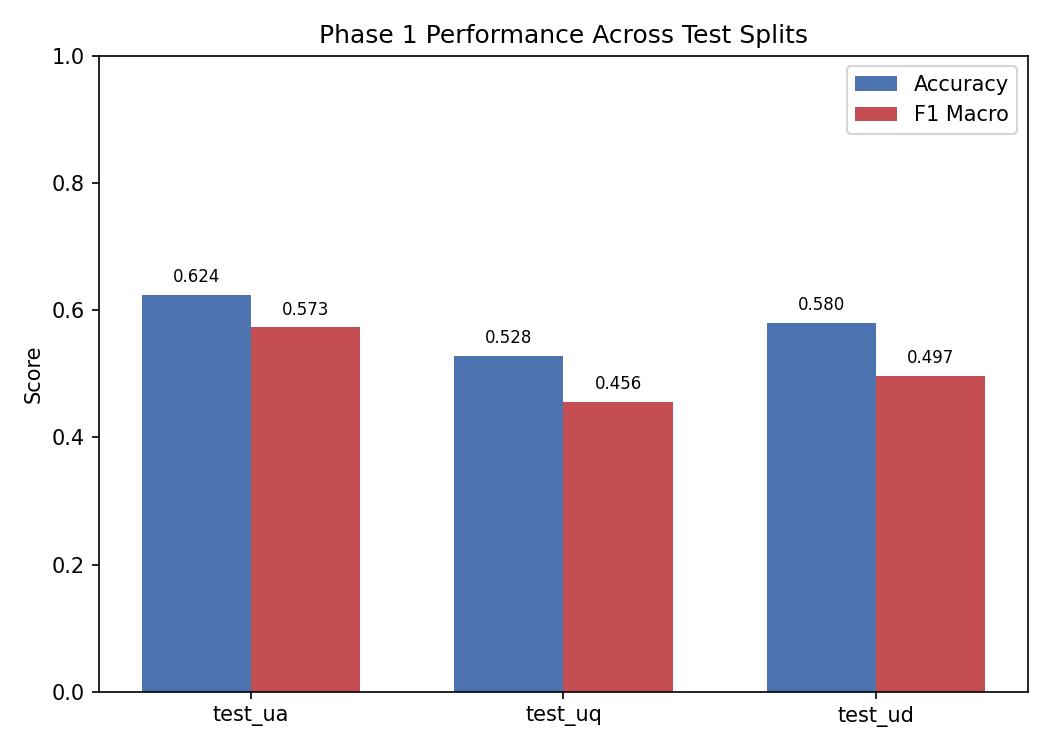
\includegraphics[width=\columnwidth]{../phase1/evaluation/accuracy_comparison.png}
    \caption{Accuracy and F1 Macro comparison across all three test splits (UA, UQ, UD). The consistent F1 drop from UA to UD confirms domain-bounded vocabulary memorisation.}
\end{figure}

\subsection{Visual Analysis}
Fig.~2 shows the label distribution across splits, revealing a strong class imbalance (Correct $\gg$ Contradictory). Fig.~3 shows the TF-IDF feature importance, where specific scientific nouns (e.g.\ ``energy'', ``circuit'') dominate the decision boundary, confirming the model memorises keywords rather than understanding logic. Figs.~4--6 show confusion matrices across all three test splits.

\begin{figure}[H]
    \centering
    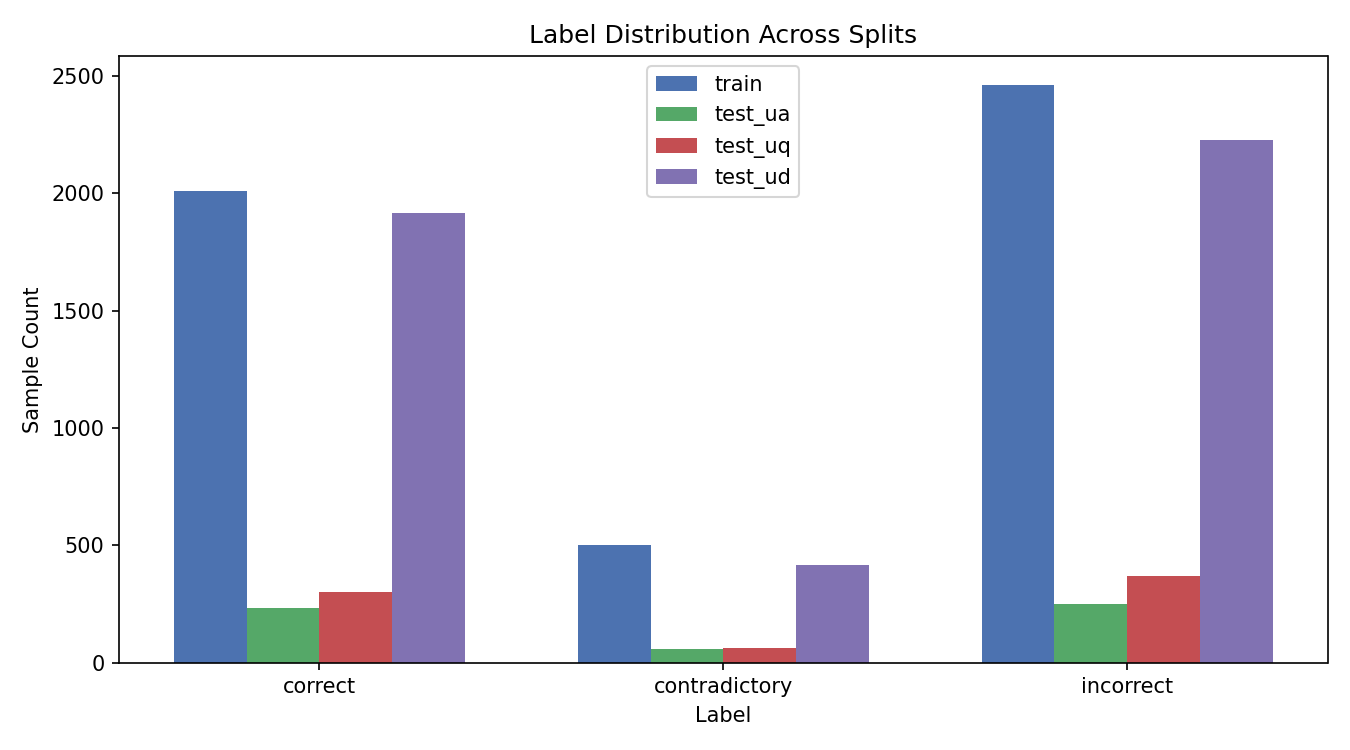
\includegraphics[width=\columnwidth]{../phase1/evaluation/label_distribution.png}
    \caption{Label distribution across train, UA, UQ, and UD splits. The class imbalance (Correct $\gg$ Contradictory) motivates inverse-frequency class weighting in the classifier.}
\end{figure}

\begin{figure}[H]
    \centering
    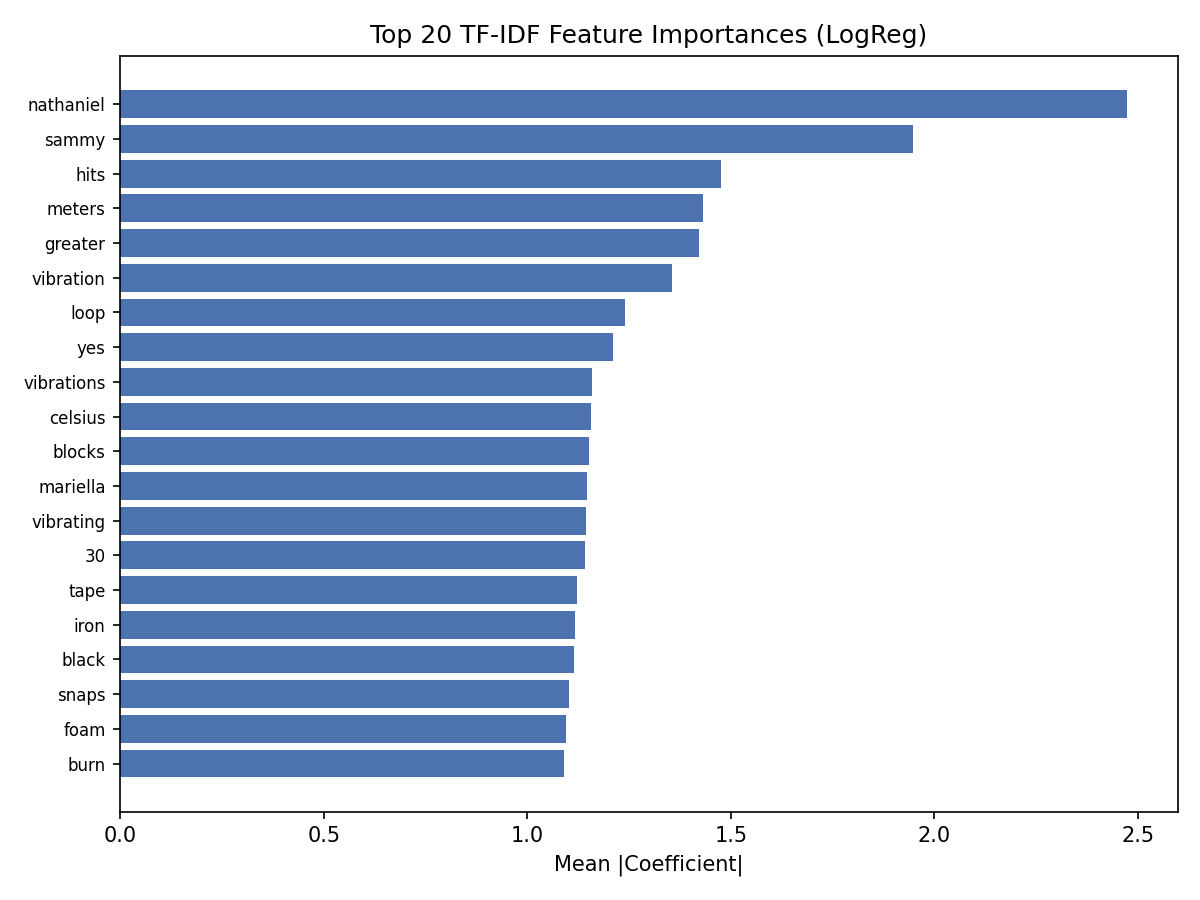
\includegraphics[width=\columnwidth]{../phase1/evaluation/feature_importance.png}
    \caption{Top 20 TF-IDF features by LogReg coefficient magnitude. Domain-specific science terms dominate, confirming vocabulary memorisation rather than conceptual understanding.}
\end{figure}

\begin{figure}[H]
    \centering
    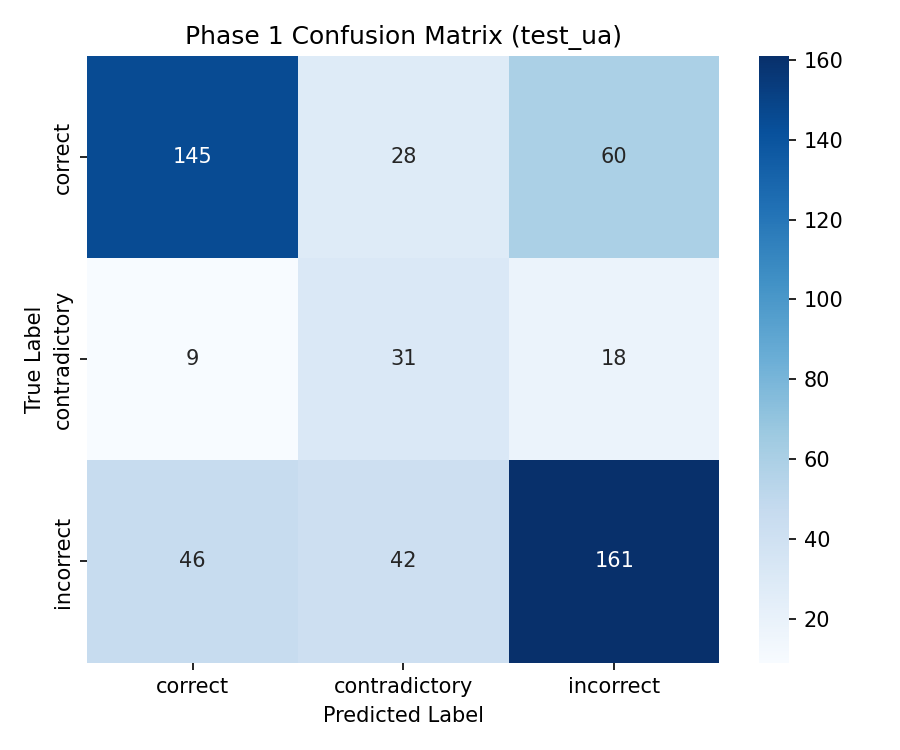
\includegraphics[width=0.32\columnwidth]{../phase1/evaluation/confusion_matrix.png}\hfill
    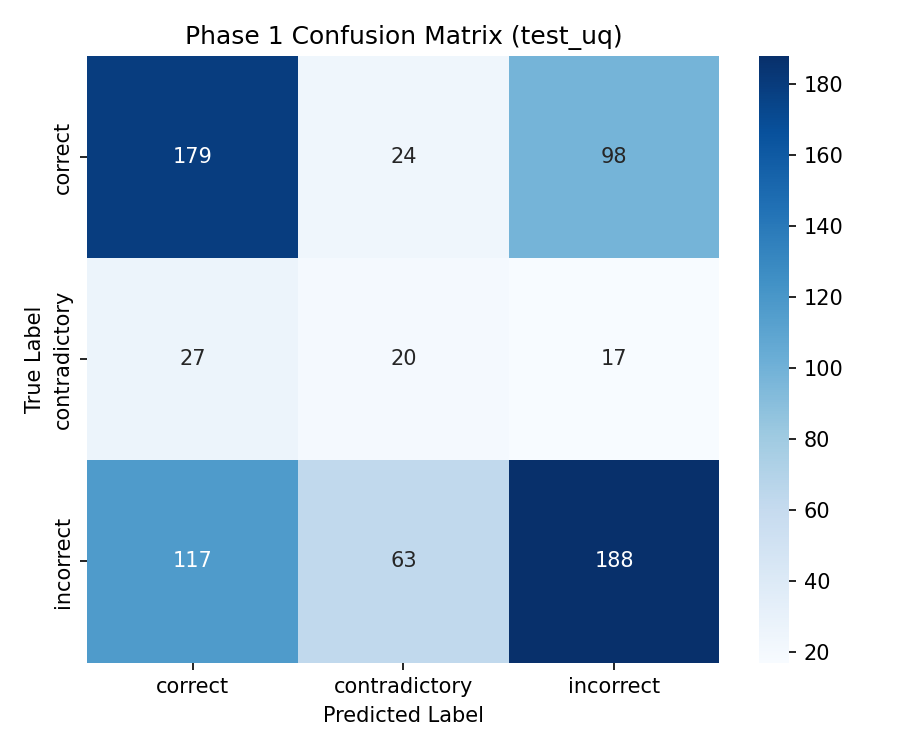
\includegraphics[width=0.32\columnwidth]{../phase1/evaluation/confusion_matrix_test_uq.png}\hfill
    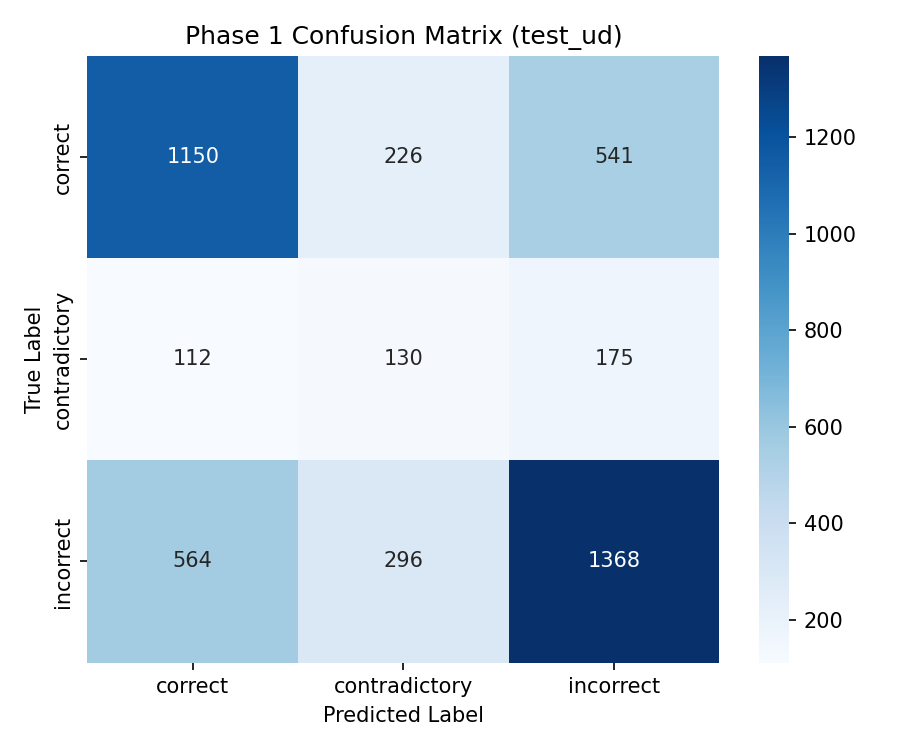
\includegraphics[width=0.32\columnwidth]{../phase1/evaluation/confusion_matrix_test_ud.png}
    \caption{Confusion matrices for (a) UA, (b) UQ, and (c) UD splits. Note the increasing off-diagonal errors from UA$\to$UD, reflecting vocabulary drift to unseen science domains.}
\end{figure}

\section{Ablation and Failure Analysis}
\subsection{The Jaccard Bottleneck}
Mathematical analysis of failure cases reveals a persistent "Jaccard Bottleneck." When a student provides a semantically perfect answer using synonyms, $J(S,R) \to 0$ in the classical space. For example:
Reference: "Produces energy."
Student: "Generates power."
Lexical Match: $0\%$.

\subsection{The UD Domain Shift}
The F1 Macro drop from UA (0.57) to UD (0.49) is a direct result of Lexical Drift. TF-IDF features are domain-bound; a model trained on biology terms fails on physics terms because their intersection is the empty set.

\section{Conclusion}
Phase 1 successfully establishes a controlled, non-neural baseline. We quantified that classical methods achieve $\approx 50-60\%$ F1 Macro but are fundamentally capped by the Semantic Gap. These findings provide a rigorous empirical justification for the neural upgrade in Phase 2.

\bibliographystyle{IEEEtran}
\begin{thebibliography}{10}

\bibitem{dzikovska2013} M. Dzikovska et al., "Semeval-2013 task 7: The joint student response analysis," \textit{Proc. SemEval}, 2013.
\bibitem{salton1988} G. Salton and C. Buckley, "Term-weighting approaches in automatic text retrieval," \textit{Inf. Process. Manage.}, 1988.
\bibitem{robertson2009} S. Robertson and H. Zaragoza, "The Probabilistic Relevance Framework: BM25 and Beyond," \textit{Found. Trends Inf. Retr.}, 2009.
\bibitem{mohler2009} M. Mohler and R. Mihalcea, "Text-to-text semantic similarity for automatic short answer grading," \textit{Proc. EACL}, 2009.
\bibitem{smith2007} R. Smith, "An Overview of the Tesseract OCR Engine," \textit{Proc. ICDAR}, 2007.

\end{thebibliography}

\end{document}
